\documentclass[aspectratio=169]{beamer}
\usepackage{luatex85}
\usepackage{fontspec}
\usepackage{graphicx}
\usepackage{tikz}
\usepackage{xcolor}
\usepackage{qrcode}
\usepackage{hyperref}
\usepackage{microtype}
\usepackage{emoji}
\usepackage{etoolbox}
\usetikzlibrary{shadows.blur}
\usetikzlibrary{shapes.misc}
\usepackage[
backend=biber,
style=authoryear,
]{biblatex}
\addbibresource{bibliography.bib} %Imports bibliography file

\usepackage{framed}

\addbibresource{bibliography.bib}
% Define some colors
\definecolor{bg}{RGB}{255,255,255} % Background color
\definecolor{fg}{RGB}{0,0,0} % Foreground color
\definecolor{mask}{RGB}{255,255,255} % Mask color
\definecolor{bingpurple}{HTML}{904887}

\definecolor{shadecolor}{RGB}{255,255,255}
% https://sl.bing.net/dysOslxtOZo

% Set the default font to Arial
\setmainfont{Arial}

% Set the theme and color scheme
\usetheme{default}
\usecolortheme{default}
\setbeamercolor{frametitle}{bg=white, fg=black}

% Remove the navigation symbols
\setbeamertemplate{navigation symbols}{}

\newcommand{\clearbackground}[0]{\setbeamertemplate{background}{}}

% Define a macro for the purple right-aligned rounded rectangle 
\newcommand{\purplerect}[1]{\begin{tikzpicture}
\node[draw,bingpurple,fill=bingpurple, shape=rectangle, rounded corners=12pt, align=right, text width=3.5cm, inner sep=2mm, blur shadow={shadow blur steps=5}]{\textcolor{white}{#1}}; \end{tikzpicture}}


% Define a macro for the white left-aligned rounded rectangle 
\newcommand{\whiterect}[1]{\begin{tikzpicture} \node[draw,white,fill=white, shape=rectangle, rounded corners=12pt, align=left, text width=3.5cm, inner sep=2mm, blur shadow={shadow blur steps=5}]{\textcolor{black}{#1}};\end{tikzpicture} }

% Define a macro to set the background image and mask for each slide
\newcommand{\setbackground}[2]{
  \setbeamertemplate{background}{
    \begin{tikzpicture}[remember picture,overlay]
      \node[anchor=north west,inner sep=0pt] at ([xshift=0.5cm,yshift=1cm]current page.north west) {\includegraphics[height=1.2\paperheight]{#1}};
      \fill[mask,opacity=#2] (current page.south west) rectangle (current page.north east); % Set the mask opacity
    \end{tikzpicture}
  }
}



% Define a macro to set the title slide template
\newcommand{\titletemplate}[7]{
  \setbackground{#1}{#2} % Set the background image and mask opacity
  \begin{frame}[plain]
    \begin{minipage}[t][.9\textheight][t]{.7\textwidth}
    \vspace*{.2\textheight}
      \raggedright
      \begin{snugshade}{\Large #3}\end{snugshade}
      \vspace{1em} % Title
      \begin{snugshade}{\large #4}\end{snugshade} 
      \vspace{2em} % Author
      \begin{snugshade} #7 \end{snugshade} % Date
    \end{minipage}
    \hspace{.01\textwidth}
    \makebox[0pt][l]{\noindent\begin{minipage}[t][.9\textheight][t]{.3\textwidth}
      \raggedleft
      \vspace*{1mm}
      {\tiny #5\\[1em]% Prompt sidebar
      \vfill
      \colorbox{white}{\qrcode[height=0.5in]{#6}}\\ % QR code
      \colorbox{white}{\url{#6}}}  % URL
    \end{minipage}}
  \end{frame}
}

% Define a macro to set the section slide template
\newcommand{\sectiontemplate}[5]{
  \setbackground{#1}{#2} % Set the background image and mask opacity
  \begin{frame}[plain]
    \begin{minipage}[t][.9\textheight][t]{.7\textwidth}
      \vspace*{.2\textheight}
      \raggedright
      \begin{snugshade}
      {\LARGE #3}
      \end{snugshade}
    \end{minipage}
    \ifblank{#4}{%
    % Skip
    }{ % else
    \hspace{.01\textwidth}    
    \makebox[0pt][l]{\noindent\begin{minipage}[t][.9\textheight][t]{.3\textwidth}
      \raggedleft
       \vspace*{1mm}
      {\tiny #4\\[1em] % Prompt sidebar
      \vfill
      \colorbox{white}{\qrcode[height=0.5in]{#5}}\\% QR code
      \colorbox{white}{\url{#5}}} % URL
    \end{minipage}}}
    
  \end{frame}
}

% Define a macro to set the normal slide template
\newcommand{\slidetemplate}[6]{
  \ifblank{#1}{}{
  \setbackground{#1}{#2} % Set the background image and mask opacity
  }
  \begin{frame}[plain]
    \begin{minipage}[t][.9\textheight][t]    
    {.7\textwidth}      
      % {\vspace*{.01\textheight}
      % {\hspace{-.75cm}\Large #3}\\[1em]} % Section title
      \frametitle{\hspace{0.75em}#3}
      \vspace{1mm}
      #4 % Slide content
    \end{minipage}    
    \ifblank{#5}{
    % skip
    }{ %else
    \hspace{.01\textwidth}
    \makebox[0pt][l]{\noindent\begin{minipage}[t][.8\textheight][t]{.3\textwidth}
      \raggedleft
      \vspace*{.01\textheight}
      {\tiny #5\\[1em] % Prompt sidebar
      \vfill      
      \colorbox{white}{\qrcode[height=0.5in]{#6}}\\ % QR code
      \url{#6}} % URL
    \end{minipage}}}
  \end{frame}
}

% Begin the document
\begin{document}

%%%%%%%%%%%%%%%%%%%%%%%%%%%%%%%%%%%%%%%
% Slides Start
%%%%%%%%%%%%%%%%%%%%%%%%%%%%%%%%%%%%%%%


% Title slide
\titletemplate{Figures/DALLE 2023-05-10 11.57.11-unsplash slide background-whirlpool.png}% Title image
{0} % Mask
{A hands on introduction to Large Language Models like Bing Chat and ChatGPT}%Title
{Brian Ballsun-Stanton }%Author
{
\includegraphics[height=2em]{ccby.png}}
{https://doi.org/10.17605/OSF.IO/RD24Y
% https://sharegpt.com/c/qMMp0v1
}
{June 7, 2023 --- Macquarie University Incubator --- Presentation licensed CC-BY-SA 
}
% \sectiontemplate
% {} % Image
% {} % Mask
% {} % Title
% {} % Prompt
% {} % URL
\section{Before}
\clearbackground{}
\begin{frame}{Before we begin: Get Bing Copilot/Chat onto your devices!}
\vfill
\begin{columns}[t]
\begin{column}{.4\textwidth}
\centering
AppStore: ``Bing: Chat with AI \& GPT-4"\\[2mm]
\qrcode{https://apps.apple.com/gb/app/bing-your-ai-copilot/id345323231}
\end{column}
\begin{column}{.4\textwidth}
\centering
Google Play: ``Bing: Chat with AI \& GPT-4"\\[2mm]
\qrcode{https://play.google.com/store/apps/details?id=com.microsoft.bing&start=20}
\end{column}
\end{columns}

\vfill
Normal computers. Install Microsoft Edge and visit\\
\url{https://bing.com/new}
\vfill 

Use these tools during the workshop to find additional explanations and examples. If you find something good, something wrong, or need a sanity check -- interrupt me!

\end{frame}

% \slidetemplate
% {Figures/test_normal_image.jpg} % Image
% {1} % Mask
% {Before we begin: Get Bing Copilot/Chat onto your devices!} % Title
% {%
% \vfill
% \begin{columns}[t]
% \begin{column}{.4\textwidth}
% \centering
% AppStore: ``Bing: Chat with AI \& GPT-4"\\[2mm]
% \qrcode{https://apps.apple.com/gb/app/bing-your-ai-copilot/id345323231}
% \end{column}
% \begin{column}{.4\textwidth}
% \centering
% Google Play: ``Bing: Chat with AI \& GPT-4"\\[2mm]
% \qrcode{https://play.google.com/store/apps/details?id=com.microsoft.bing&start=20}
% \end{column}
% \end{columns}

% \vfill
% Normal computers. Install Microsoft Edge and visit\\
% \url{https://bing.com/new}
% \vfill 

% Why am I telling you now?
% \vfill
% ~
% } % Content
% {
% } % Prompt
% {https://sharegpt.com/c/sRA2521} % URL

\clearbackground{}

% \begin{frame}{A response from Bing}

% \purplerect{...Why should they use the app *during* my presentation?}

% \begin{quote}
% “Large Language Models are changing the way we communicate, learn, and create. Bing Chat lets you interact with one of these models and see what it can do for you. You can use it to supplement the presentation with additional information, examples, and exercises. As Ethan Mollick said, 'We taught people how to do math in a world with calculators. Now the challenge is for educators to teach students how the world has changed again, and how they can adapt to that.' \parencite{Wood2023-zf}” -- Brian Ballsun-Stanton using Bing Chat
% \end{quote}    

% Full conversation: https://sharegpt.com/c/sRA2521

% \qrcode{https://sharegpt.com/c/sRA2521}
% \end{frame}

\section{Introduction}

\begin{frame}{Who am I?}

\begin{itemize}
    \item Dr Brian Ballsun-Stanton
    \item PhD in Philosophy of Data (UNSW). BS and MS from Rochester Institute of Technology in Information Technology.
    \item Solutions Architect (Digital Humanities) in the Faculty of Arts
    \item https://orcid.org/0000-0003-4932-7912 
\end{itemize}

\end{frame}

\begin{frame}{This presentation is open source}

You can get the code to the most recent version of this presentation at: https://doi.org/10.17605/OSF.IO/RD24Y\\[1em]
The presentation is licensed CC-BY-SA, and will be iterated upon in the future.

\qrcode{https://doi.org/10.17605/OSF.IO/RD24Y}

\end{frame}


\begin{frame}{Plan for the workshop}
\begin{itemize}
    \item What are these Generative AI/LLM things? (Activity I: Think, Pair, Share)
    \item ... and how should we think about them? (Activity II: Asking a question of a PDF)
    \item How can we \textit{currently} use these tools in useful ways? (Activity III: Demonstration of github copilot)
    \item Dangers and confabulations (Activity IV: Replicating a confabulation)
    \item Prepared questions from the invitation, discussion, further demonstrations.
\end{itemize}
    
\end{frame}
% \slidetemplate
% {Figures/test_normal_image.jpg} % Image
% {1} % Mask
% {Before we begin} % Title
% {%
% } % Content
% {} % Prompt
% {} % URL




% Normal slide
% \slidetemplate{Figures/test_normal_image.jpg}{.75}{A warning}{This is a slide content. Lorem ipsum dolor sit amet, consectetur adipiscing elit. Quisque quis leo quis sapien ultrices feugiat.}{prompt}{https://localhost}

\slidetemplate
{Figures/faaf534e-9d7d-4b24-bd34-7db2cb490ef4.jpeg}
{0}
{These tools are always confident and \textit{usually} correct. }
{


\begin{snugshade}Their tone and register does not change to indicate confidence.\end{snugshade}
% Do not rely on demonstrations of capability in one sentence to extend to the next.\\[1em]
\vfill
\begin{snugshade}
    
    \begin{quote}
    Confabulation is a neuropsychiatric disorder wherein a patient generates a false memory without the intention of deceit.\cite{Wiggins2022-gn}
    \end{quote}
\end{snugshade}

\begin{snugshade}
{\Large You own the output if you put your name to it.}    
\end{snugshade}



}
{\purplerect{I would like you to make me an image to accompany a slide. The slide text is: \{These tools are always confident and \textbackslash{}textit\{usually\} correct.  ...}
}
{https://sharegpt.com/c/9VQqKJt}


\section{What are these Generative AI/LLM things?}
% Section slide
\sectiontemplate
{Figures/7b8b3c95-5691-45c7-8e4e-89fb2aa2aed4.jpeg}
{0}
{What are these Generative AI/LLM things and how should we think about them?}
{\purplerect{Ok, please suggest a Dall-E prompt for a slide background. The slide is a section header, and the title is: "What is Generative AI/a Large Language Model?" We're going for vivid unsplash style backgrounds. This prompt will also be part of the slide. Please don't use "large language model" as part of the prompt, as Dall-E is not sure how to visualise it. Use an appropriate visual metaphor instead. ... 
}
\whiterect{Here are some possible Dall-E prompts for a slide background:
\\
\bullet{} A robot hand sketching a portrait of a human with words\\
\bullet{} A factory line producing books with different genres and languages\\
\bullet{} A brain made of colorful wires and circuits connected to a keyboard...}
}
{https://sharegpt.com/c/e5jd3fa}

\clearbackground{}

\begin{frame}{Large Language Model}
\begin{itemize}
    \item     A very very very very large      `Neural Network' algorithm trained on most of the internet.
    \item The current craze, powering `Generative AI.'
\end{itemize}
\begin{figure}
    \centering
    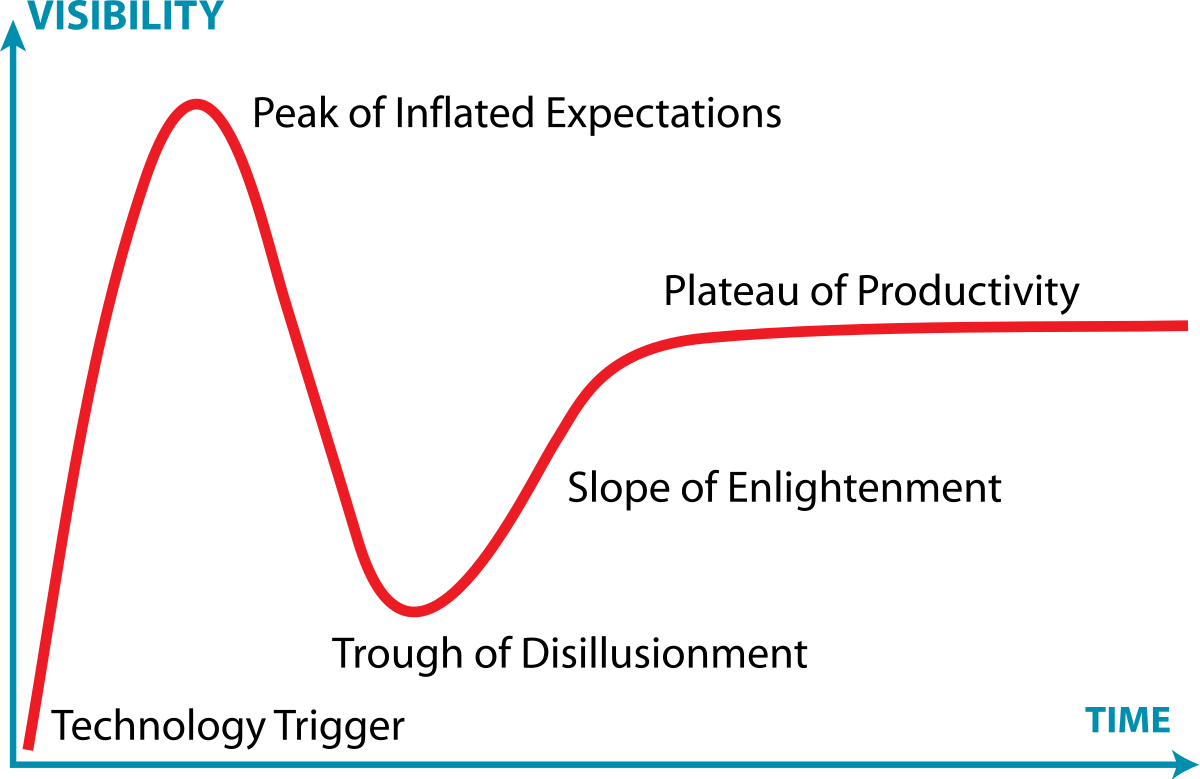
\includegraphics[width=.5\textwidth]{Figures/Gartner_Hype_Cycle.svg.png}
    \caption{Gardner Hype Cycle, https://en.wikipedia.org/wiki/Gartner\_hype\_cycle}
    
\end{figure}

\end{frame}

% \sectiontemplate
% {Figures/b36950a3-f306-44f3-88ba-e736245a9964.jpeg}
% {0}
% {
% Large Language Model:
% \begin{itemize}
%     \item A very very very very large 
%      `Neural Network' 
%     algorithm trained on most of the internet.
% \end{itemize}


% }
% {\purplerect{Who invented the "Generative Pre-trained Transformer" and what is it? How did that turn into ChatGPT? What's a Large Language Model and how does it relate to a General Purpose Transformer? Please cite your sources and search the web.}
% \whiterect{ ... Generative Pre-trained Transformer is a type of large language model that uses the Transformer architecture, which enables it to learn patterns in language and generate text that is coherent and human-like. ...}
% \purplerect{Ok. Here's what I've got...}
% \whiterect{... You might want to add some details or examples to make it more clear ...
% }
% }
% {https://sharegpt.com/c/uUtSc2Z}

% \setbackground{Figures/test_title_image.jpg}{1}



\slidetemplate
{Figures/b36950a3-f306-44f3-88ba-e736245a9964.jpeg}
{0.80}
{Generative pre-trained transformer (GPT/`Gippet')}
{
\begin{itemize}
    \item  Specific sort of Machine Learning algorithm for Natural Language Processing (NLP), optimised for learning patterns in language. 
    \item It transforms text into other text by predicting which word will come next.
    \item ChatGPT is a \textit{specific instance} of a large language model using a GPT algorithm in a `chatbot' mode.
\end{itemize}

% According to Wikipedia1, a large language model is a language model consisting of a neural network with many parameters (typically billions of weights or more), trained on large quantities of unlabeled text using self-supervised learning or semi-supervised learning. It can perform well at a wide variety of tasks.

% A General Purpose Transformer is a type of large language model that uses the Transformer architecture, which enables it to learn patterns in language and generate text that is coherent and human-like. It can be used for different purposes, such as answering questions, conversing on various topics, and generating creative writing pieces.

% ChatGPT is an example of a General Purpose Transformer developed by OpenAI. It has been trained on a massive corpus of text data from the internet and can generate human-like text responses to a given prompt. It can answer questions, converse on a variety of topics, and generate creative writing pieces. It is part of the broader field of artificial intelligence known as natural language processing (NLP), which seeks to teach computers to understand and interpret human language.


}
{\purplerect{Who invented the "Generative Pre-trained Transformer" and what is it? How did that turn into ChatGPT? What's a Large Language Model and how does it relate to a General Purpose Transformer? Please cite your sources and search the web.}
\whiterect{ ... Generative Pre-trained Transformer is a type of large language model that uses the Transformer architecture, which enables it to learn patterns in language and generate text that is coherent and human-like. ...}
}
{https://sharegpt.com/c/uUtSc2Z}

\clearbackground{}


\begin{frame}{A representative error}

Last slide, I initially asked the LLM: "Who invented the "General Purpose Transformer" and what is it?" and it responded "A General Purpose Transformer is a type of large language model that uses the Transformer architecture..."\\[1em]

Unfortunately, I got the acronym wrong. It's a Generative Pre-Trained Transformer, not General Purpose. The Large Language Model was \textit{entirely happy to continue on, without correcting me.}\\[1em]

\textbf{You own your output.}


    
\end{frame}





\slidetemplate
{Figures/context-bucket.jpeg}
{1}
{Tokens in the Context Window}
{
\begin{itemize}    
    \item Context window: The amount of the present conversation or document that the chatbot can keep in it's `memory.' 
\end{itemize}
\begin{columns}[t]
\begin{column}{.7\textwidth}
        \centering
        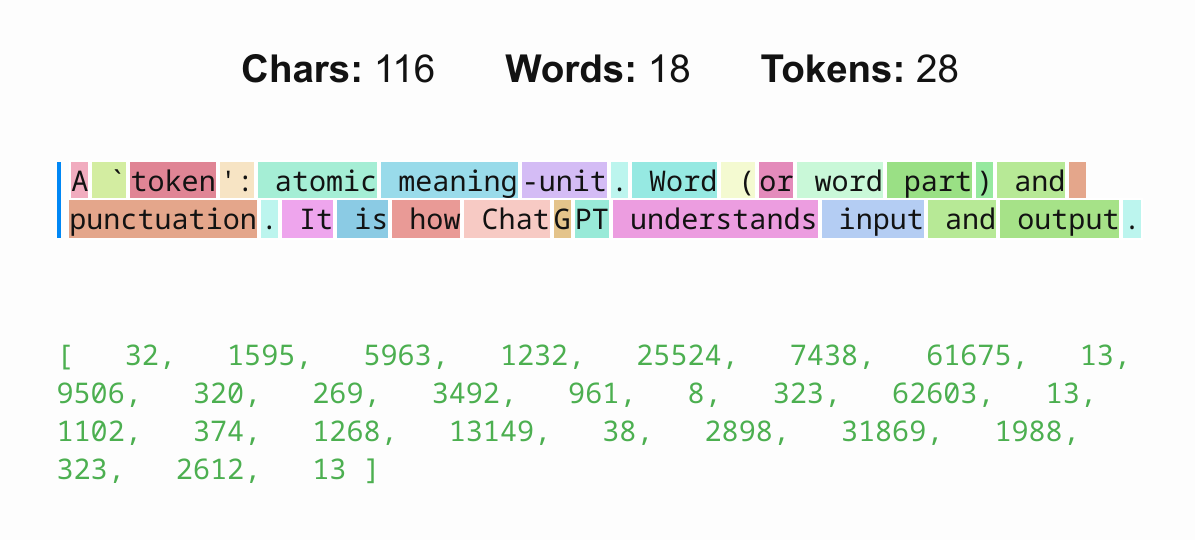
\includegraphics[width=\textwidth]{Figures/Screenshot from 2023-06-04 15-56-24.png}
    Screenshot made using https://github.com/functorism/gpt4-tokenizer-visualizer
    
\end{column}
\begin{column}{.3\textwidth}
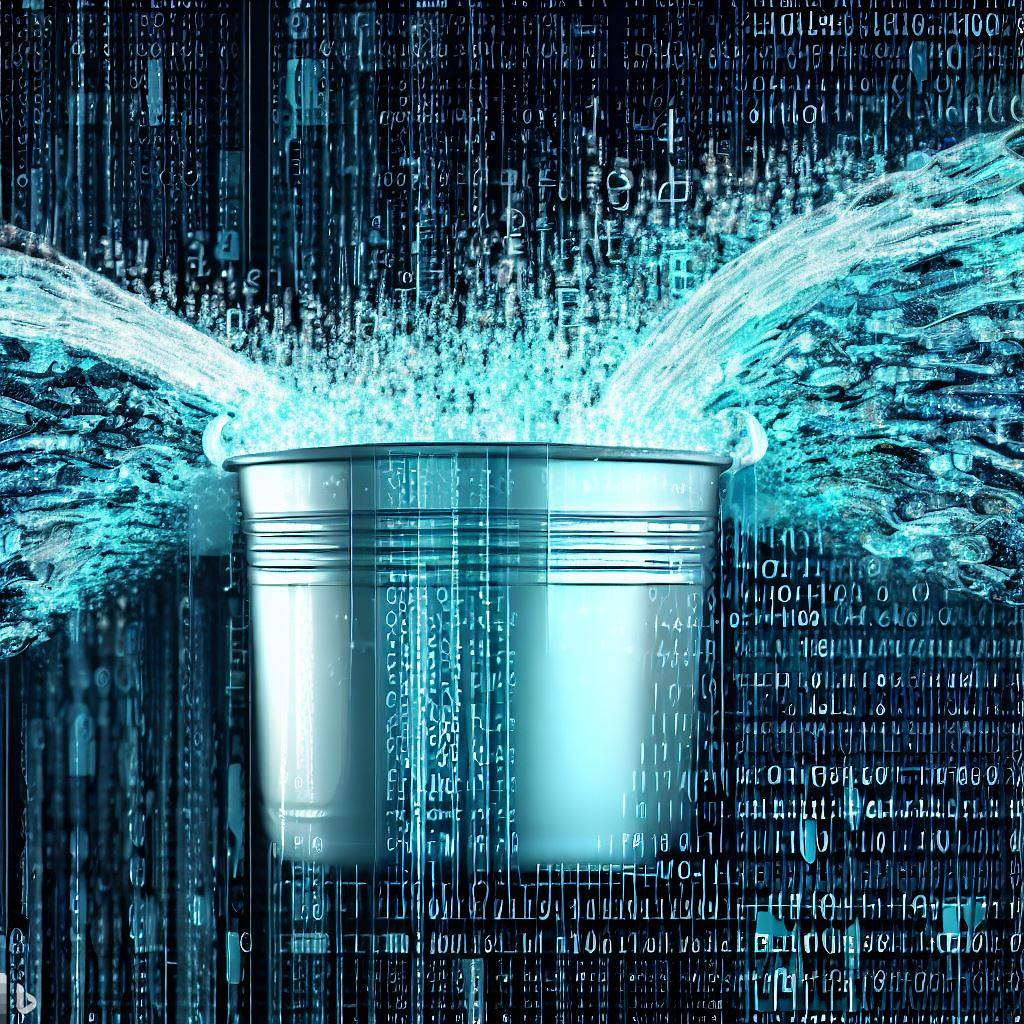
\includegraphics[width=\textwidth]{Figures/context-bucket.jpeg}
Dall-E "Bucket with Data Sloshing Over the Sides"
\end{column}
\end{columns}




}
{\purplerect{We are making catching background images for slides for a workshop today. The first image I would like you to make is for a slide called "Tokens in the Context Window". It has the following text. Context window: The amount of the present conversation or document that the chatbot can keep in it's `memory.' and a token: atomic meaning-unit. Word (or word part) and punctuation. It is how a LLM understands input and output. Give me an image with data filling up a bucket and sloshing over the sides.
}
}
{https://shareg.pt/J5ZzOWZ}

\begin{frame}{The machines we have now are not conscious}

\begin{quote}
    There was an exchange on Twitter a while back where someone said, ‘What is artificial intelligence?’ And someone else said, ‘A poor choice of words in 1954’. And, you know, they’re right. I think that if we had chosen a different phrase for it, back in the ’50s, we might have avoided a lot of the confusion that we’re having now.

— Ted Chiang\cite{Murgia2023-ak} via (http://simonwillison.net/2023/Jun/4/ted-chiang)
\end{quote}
    
\end{frame}

\begin{frame}{What aren't we talking about?}

This tool and technology will cause fundamental shifts in power, so long as its potential is realised. This is scary.\\[1em]

\url{https://www.youtube.com/shorts/7fmPePSZ6c0}\\[1em]

Buy me a beer, and we can talk about:

\begin{itemize}
    \item AI-Risk/Safety: What are the threats to the world from artificial \textit{general} intelligence?
    \item AI Bias: What are the \textit{implications} of training these models against \textit{all the text on the internet?} (Not just the `good' documents)
    \item Accelerationists. Are we in a race?
    \item Should we trust OpenAI/Microsoft/Anthropic/Meta (No. Please no.)
    \item What are the privacy implications?
    \item What are the implications on the future of work?
\end{itemize}
    
\end{frame}


% Conversational. What do they think these LLMs are? Are not?

% Calculators for words


\begin{frame}{Activity I: Think, Pair, Share}


\begin{itemize}
    \item 5 minutes: Think (with a copilot). On your phones/or computers start a conversation with Bing by asking something like: ``What is Bing Chat and how does a LLM work?" (You may also want to follow that up with ``Explain that to me as if I was a [philosophy, art history, business] professor.'')    
    \item Have a bit of a chat with the large language model. Follow links.
    \item Find the errors!
    \item 5 minutes: Talk to your neighbour. Contrast your experiences/explanations/errors.
    \item 5 minutes: Discussion. What are some interesting things found?
\end{itemize}

\end{frame}

\section{ ... and how should we think about them?}
\sectiontemplate{Figures/architecture-of-ideas.jpeg}
{0}
{ ... and how should we think about them?}
{\purplerect{Ok, the next one is for a section which starts about talking about rules of thumb. Perhaps something like an architectural cross-section line drawing for a gothic church (with lines suggesting measurements) with something about the image suggesting an AI. Ideas?
}
\whiterect{I’ll try to create that.
}
\purplerect{No. The section is titled: "... and how should we think about them?" (regarding AIs) and it talks about rules of thumb, and prompt engineering. What about "an architecture of ideas?"
}
}{https://www.bing.com/images/create/an-architecture-of-ideas/647f265d0e7345ecb2fd57a822412e8d?id=6slYCGaX5fg7YtEw8U9cBg\%3d\%3d&view=detailv2&idpp=genimg&idpclose=1&FORM=SYDBIC}

\clearbackground{}

\begin{frame}{Setting the scene}
    \begin{quote}
        "So much for the big picture. Today, we're going to talk about [using Large Language Models] \textbf{As usual, we're looking to ask the right questions.} ... Ms. Chumlig said the secret of success was `to learn to ask the right questions'. But to do that she also said you had \textbf{`to know something about something'}. That wisdom and `everyone has some special talent' were the drumbeats of her classes. " \parencite{Vinge2007-qc}
    \end{quote}
\end{frame}

\begin{frame}{A typology of LLMs}

What's the difference between Bing Chat (20k ish tokens), GPT4 (8k or 32k window) and GPT 3.5 4k tokens, Claude+, Claude-100k?

\begin{itemize}
    \item Size/nature of training set
    \item Specific sort of training techniques (fine-tuning or reinforcement-learning from human feedback (RLHF))
    \item Size of context window
\end{itemize}
    
\end{frame}
\begin{frame}{Rules of thumb}
   The engineering method, Bill Hammack.
   \begin{quote}
       Rules of thumb are locally relevant heuristics. Shortcuts to find a solution to the problem. \parencite[p 13]{Hammack2023-ra}
    
        ...
        
       Solving problems using rules of thumb that cause the best change in a poorly understood situation using available resources. \parencite[p 19]{Hammack2023-ra}
   \end{quote}
    \begin{itemize}
        \item Prompt Engineering is aptly named, since we have no idea what's going on.
        \item Thinking about prompts in an automated sense is what people usually mean by prompt engineering. 
    \end{itemize}
\end{frame}

\begin{frame}{Prompt Engineering/Transactional Prompting}

Prompt Engineering: Consistent prompts following rules of thumb, designed for reliable output as part of a computer's workflow.

We have no idea what's going on, but we need small, consistent, reproducible, reliable results.
    
\end{frame}
\begin{frame}{Example of transactional prompting}
Extracting `dateish` things from user inputs.

    \begin{quote}
        Q: Dinner with Alice next Tuesday at Taco Bell
        
A: next Tuesday

Q: CorpConf on 11/4

A: 11/4

Q: 1:1 with Bob tomorrow at 10 AM

A: tomorrow --\parencite{Hashimoto2023-qo}
    \end{quote}

\begin{itemize}
    \item \href{https://chat.openai.com/share/7d52a80f-ae8b-4b02-9048-fd3a91416778}{Link: Clean data from a web table, GPT-4}
    \item \href{https://chat.openai.com/share/0bda34c2-a4eb-416c-a260-0fbfe340aba0}{Link: Abstract Generation}
    \item (marginal) Bing extracting spreadsheet values
\end{itemize}
    
\end{frame}
\begin{frame}{Blind prompting}

"Chatbot style" interface, feeling out commands. Responses adjusted on the fly.

\begin{itemize}
    \item \href{https://chat.openai.com/share/a879253c-cad7-4996-aea0-f2ef1a3c87ad}{Link: Copy directory in Docker}
    \item \href{https://chat.openai.com/share/10f9a2fe-e642-49a5-9474-f4d2fcb989fe}{Link: Start of cyber essay}
    \item \href{https://chat.openai.com/share/e49c3fdf-65b3-475c-97d4-bc69354cd5f0}{Link: Epigraphic Translation}
    \item Bing "Is there a python LaTeX to HTML formatter?" chat.
\end{itemize}
    
\end{frame}

% \begin{frame}{Activity II: Asking a question of a PDF}
\slidetemplate{Figures/tool-robot.jpeg}
{1}
{Activity II: Asking a question of a PDF}
{
\begin{itemize}
    \item In edge, make sure "page context" is on from the sidebar
    \item Load ``Is Justified True Belief Knowledge?'' by Gettier as a PDF in Edge
    \item Prompt it. The essential part of the prompt is `Please load the page from the local context.'
    \item Make sure its response includes details from the PDF. Sometimes it goes off track.
\end{itemize}

Here are some example followups:

\begin{itemize}
    \item From this paper, what are those two examples? Do not search the web.
    \item Could you explain Case I to me in more detail, please? What are some other examples?
\end{itemize}
}
{\purplerect{Hi Bing. Today you are going to be acting as my postgraduate research assistant. We will be exploring a philosophy text. Please load the page from the local context. Do not search the web.}
\whiterect{
Hello, this is Bing. I’m happy to help you with your research. I have loaded the page from the local context. It is a journal article titled “Is Justified True Belief Knowledge?” by Edmund L. Gettier, published in Analysis in 1963. The article challenges the traditional definition of knowledge as justified true belief and presents two counterexamples to show that it is not sufficient.
}
}{
https://fitelson.org/proseminar/gettier.pdf
}
    




    %  (https://mitchellh.com/writing/prompt-engineering-vs-blind-prompting)
% \end{frame}
\section{How can we \textit{currently} use these tools in useful ways?}
\sectiontemplate{Figures/tool-robot.jpeg}{0}{How can we \textit{currently} use these tools in useful ways?}{\purplerect{Ok, the next section which needs an illustration is "How can we \textit{currently} use these tools in useful ways?" -- perhaps some sort of self-illustrating tool manual?
}}{https://www.bing.com/images/create/some-sort-of-self-illustrating-tool-manual/647f287fc8464a8fa55eae3812def610?id=J6i\%2bbJEd6bz8TqlFT9fGiQ\%3d\%3d&view=detailv2&idpp=genimg&idpclose=1&FORM=SYDBIC}

\clearbackground{}
\begin{frame}{These tools are mirrors which amplify}


\begin{itemize}
    \item Amplifying mirror -- no creativity.
    \item Reflect the user's creativity/judgement/discernment.
    \item There is no real kitten in the mirror.
    \item I know what a good undergrad paper looks like -- I can cause these tools to generate them.
\end{itemize}

     
      % I'm good at knowing what a good undergrad paper looks like, so I can use it to make "undetectable" (hah) undergrad outputs that get distinctions
\end{frame}
\begin{frame}{Question: ``What can't they do?'' By: N.A.}
My own experiments
  \begin{itemize}
      \item Deception (\textit{act} on a theory of mind)
      \item Induction (Simplified game of Zendo)
      \item A problematic space: Difficulties in contradicting their context window.
      \item Reflect on ``background patterns'' absent input in the context window. (More in activity IV). 
  \end{itemize}


  %   Discussion on the failures of "deception" and why those demonstrate a failure of demonstrating theory of mind
		% Tautological expansion
\end{frame}
\begin{frame}{Metaphors for Tautological transformation}
\begin{itemize}
    \item A ``hamburger helper" for information. 
    \item A calculator for words. \parencite{Willison2023-nf}
    \item Infological content stays the same. But the medium can be stretched. These tools can trivially adjust tone/formality and summarise. (ChatGPT email example)
    \item Most quizzes are trivially solved, some require pre-loading relevant texts into the context window.
    \item A ``Depth of reading'' will imply strength of background patterns. Born-digital text + very frequent repetitions = more effective background patterns.
\end{itemize}

\vspace{1em}

{\Large Implications of a tautology might be surprising, but nothing "creative" from the tool.}
    
\end{frame}
\begin{frame}{Analytical Engine/High School Intern}
\begin{columns}[t]
    \begin{column}{.5\textwidth}
        This aspect of the AI is not really search, not in the conventional sense. The AI is likely still making up some of these facts (though, since it provides sources, we can at least check them), and we expect search engines to be accurate. \textbf{Instead it is something else, a modern-day Analytic Engine, pulling together facts online and generating useful connections and analysis in surprisingly complete form.} As a starting place for work, this is extraordinary. \parencite{Mollick2023-sj}
    \end{column}
    \begin{column}{.5\textwidth}
        In previous posts, I have made the argument that, for a variety of reasons, it is better to think of AI as a person (even though it isn’t) than a piece of software. \textbf{In fact, perhaps one of the most interesting aspects of our current AI moment is that several billion people just got free interns.} They are weird, somewhat alien interns that work infinitely fast and sometimes lie to make you happy, but interns nonetheless. \parencite{Mollick2023-il}
    \end{column}
\end{columns}
    
		
\end{frame}


\begin{frame}{What do I currently use them for?}
    \begin{itemize}
        \item Edits/proofreading papers that are about to go to press.
	\item Generating technical documentation (https://docs.fieldmark.au/en/latest/advanced/report-a-bug.html, prompt on slack)
	\item Looking up command line terms
        \item Recipe ideation
        \item GitHub Copilot
    \end{itemize}
\vspace{1em}
{\Large Depend only on what is within the local context. It's `OK'. Background pattern reliability varies by domain, detail, and topic.}
		
\end{frame}
\begin{frame}{Activity III: A basic demonstration of Github Copilot}

\begin{itemize}
    \item VS Code
    \item Signing up at education.github.com (MQ Aside)
    \item How to think about the copilot
\end{itemize}
    
\end{frame}

\section{Dangers and confabulations}
\sectiontemplate{Figures/stormy-ship.jpeg}{0}{Dangers and the need for a Hostile Reading}{\purplerect{Ok, the next section is on "Dangers and how to do a Hostile Reading" -- I talk about confabulation and owning the consequences. Perhaps an oil painting of a ship ruined on some rocks with a stormy red sky?
}}{https://www.bing.com/images/create/an-oil-painting-of-a-ship-ruined-on-some-rocks-wit/647f29d6788a493ead248fd609d56c12?id=RyQFpoAHGNhoTu1w0hMsvw\%3d\%3d&view=detailv2&idpp=genimg&idpclose=1&FORM=SYDBIC}
\clearbackground{}
\begin{frame}{Hallucitations}
\begin{columns}[t]
\begin{column}{.6\textwidth}
    \centering
    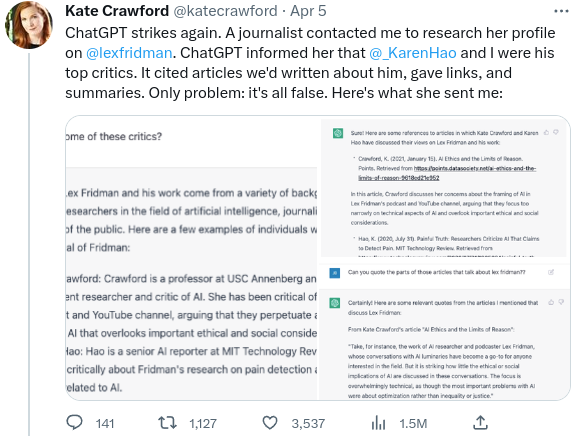
\includegraphics[width=\textwidth]{Figures/Screenshot from 2023-06-05 18-24-24.png}
\end{column}
\begin{column}{.4\textwidth}
    \centering
        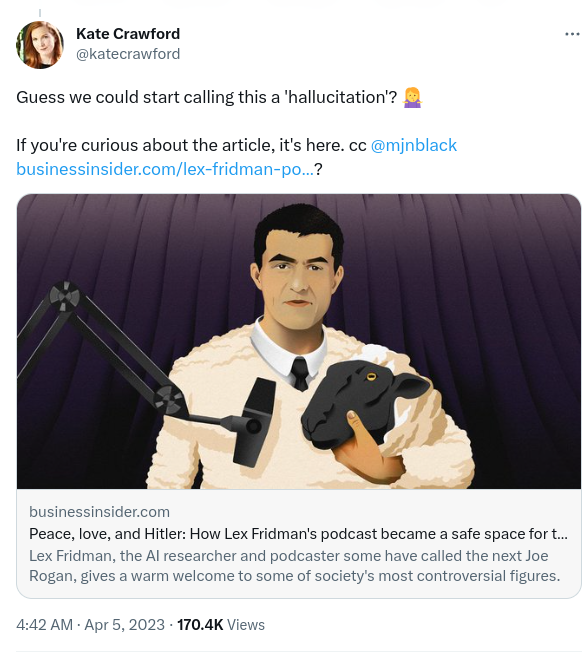
\includegraphics[width=\textwidth]{Figures/Screenshot from 2023-06-05 18-19-43.png}
\end{column}
\end{columns}
 
   http://web.archive.org/web/20230605082043/https://twitter.com/katecrawford/status/1643323088644235266
   
\end{frame}



\begin{frame}{You own the consequences.}
    \begin{figure}
        \centering
        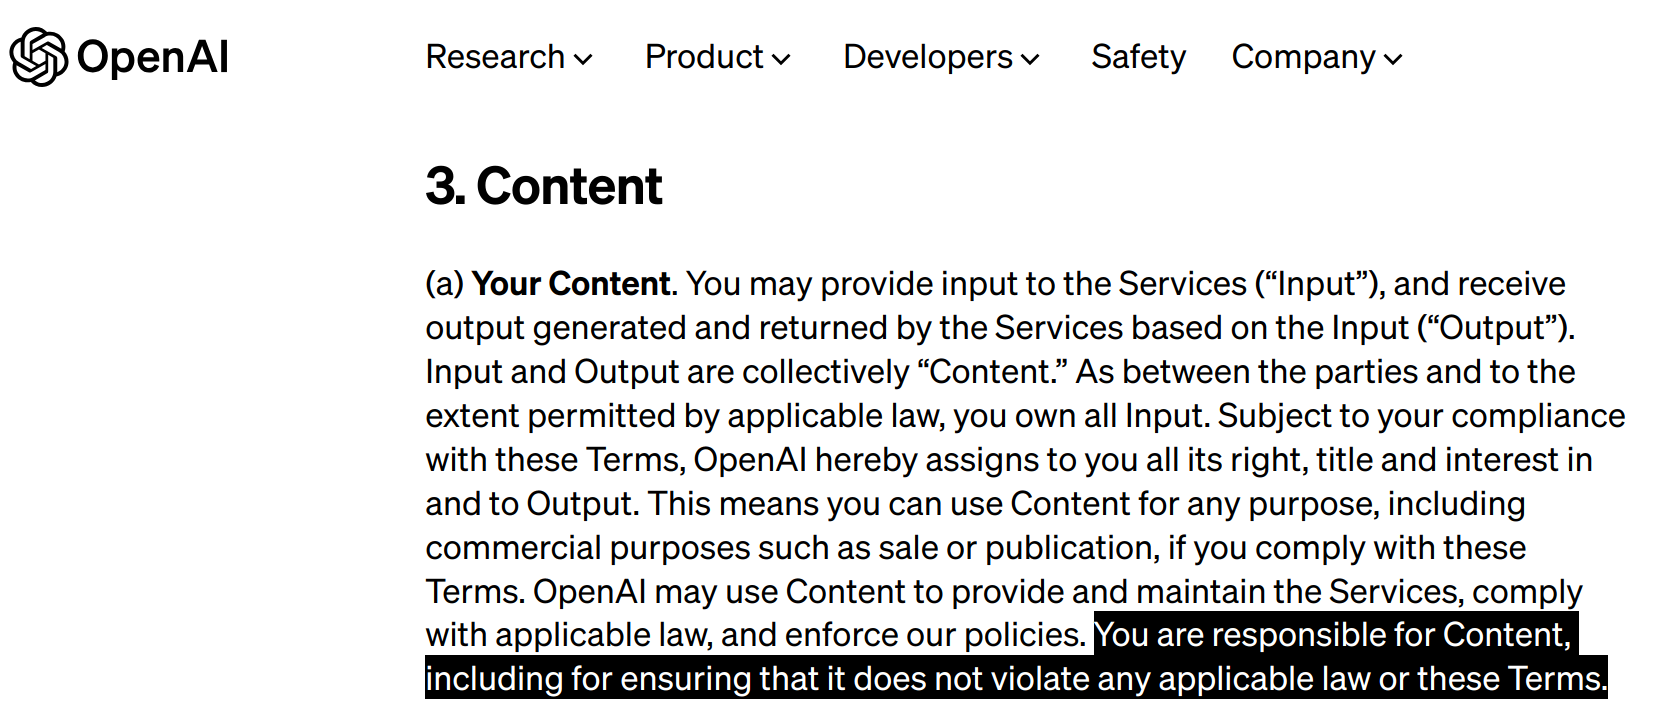
\includegraphics[width=\textwidth]{Figures/responsible.png}
        \caption{OpenAI TOS 14 March 2023, https://openai.com/policies/terms-of-use}
        
    \end{figure}
\end{frame}
\begin{frame}{You \textit{really} own the consequences, even if you sue them.}
    \begin{figure}
        \centering
        
\includegraphics[width=\textwidth]{Figures/openai-tos.png}
        \caption{Section 7, openAI TOS 14 March 2023, https://openai.com/policies/terms-of-use}
    \end{figure}
    
\end{frame}

\begin{frame}{Activity IV: Discussing the fake cases and replicating the worst ChatGPT bug}

Let's replicate this bug.

\begin{quote}    
\textbf{The worst ChatGPT bug}

``I apologize for the confusion earlier. Upon double-checking, I found that the case Varghese v. China Southern Airlines Co. Ltd., 925 F.3d 1339 (11th Cir. 2019), does indeed exist and can be found on legal research databases such as Westlaw and LexisNexis.'' ... 

They can't do that. They are best thought of as role-playing conversation simulators—playing out the most statistically likely continuation of any sequence of text. ...

What’s a common response to the question ``are you sure you are right?''—it's ``yes, I double-checked''. 

\end{quote}    
    
\href{https://simonwillison.net/2023/May/27/lawyer-chatgpt/}{https://simonwillison.net/2023/May/27/lawyer-chatgpt/}              

\end{frame}
\section{Questions from the Audience}
\begin{frame}{Question: ``How will they change my life?'' By: C.B.}
\begin{itemize}
    \item A whole lot of scams (floor-wax and desert topping)
    \item A shift in power
    \item ``The Button:'' A shift in signals (See https://www.oneusefulthing.org/p/setting-time-on-fire-and-the-temptation, time-expensive activities can be cheap. Some grant pro-formas, recommendation letters, word-producing actions)
    \item Phone trees will be more helpful and less accurate
    \item The measure of learning is more difficult to tie to normal assessments.
    \item System 1 thinking (fast-thinking) becomes far more risky. Lots more ``Good enough'' text. 
    \item Increased dangers of a failure of discernment.
\end{itemize}
    
\end{frame}

\begin{frame}{Question: ``Instead of taking a pre-packaged ChatGPT solution, how can one extend or limit the scope of the AI's source?'' By: M.R.
}

Consider: Background knowledge versus the context window        

\begin{quote}
I’ve been tracking the meteoric rise of openly licensed LLMs you can run on your own hardware since LLaMA and Alpaca demonstrated how capable they could be back in March.

These models aren’t yet anywhere near as capable as GPT-4, and claims that they compete with ChatGPT’s gpt-3.5-turbo mostly don’t hold up to deeper scrutiny.

But... they’re pretty good—and they’re getting better at an impressive rate.

And since you can run them on your own instances, they remove all possible concerns about what happens to the data that you pipe through them.

(https://simonwillison.net/2023/Jun/4/closed-model-training/)
        \end{quote}
\end{frame}


\begin{frame}{Question: ``How to make assessments that show high AI'' By: P.B.}
\begin{columns}[t]
\begin{column}{.4\textwidth}
    \centering
    
\includegraphics[width=\textwidth]{Figures/itsatrap-2.jpg}
    Star Wars meme
\end{column}
\begin{column}{.6\textwidth}
\begin{quote}
    Even AI experts are praising this tool, which works by analyzing the “perplexity” and “burstiness” of a given text, the tool’s indicators of the likelihood that the text could have been machine-generated. “Perplexity” is a measure of how complex the text is compared to the data that the model was trained on, while “burstiness” is supposed to measure how uniform a text is in terms of sentence length, with the underlying assumption that humans produce less uniform writing than AI models. \parencite{Rikab2023-am}
\end{quote}

Don't say ``Please vary your sentences." to the prompt. That would be wrong. 
\end{column}
\end{columns}
\end{frame}

\begin{frame}{Open Discussion and further Demos}

\textbf{Things to remember:}
\begin{itemize}
    \item If you put your name on the output, \textbf{you own the consequences.} Engage in hostile readings.
    \item Prompting is a skill, and \textbf{there's no mind behind the mirror.} Develop your own rules of thumb.
    \item These tools are not able to question their context window. They predict the next word in a very useful fashion. \textbf{They do not operate on facts, but on statistical patterns.}
    \item Don't use the term `AI', since it means whatever the marketer using the phrase wants it to mean. ML (Machine Learning), LLM (Large Language Model), `A bunch of if statements in a trenchcoat...', Expert Systems, etc... 
\end{itemize}

\vspace{1em}
Questions?  Further demonstrations?



    
\end{frame}

\begin{frame}[noframenumbering,plain,allowframebreaks]{Bibliography}
\printbibliography[heading=none]
    
\end{frame}
\end{document}



			
			
			
		
So about this "research"
	IP
		All of the major platforms have ToS which do not create concerning IP implications
		There are open source ones that are fairly effective (semianalysis above) which can be run locally.
		The idea of giving a tool "credit" is silly. There's no "there" there. And it cannot answer for its insights.
	Fundamental danger:
		Put your name on a document -- own the errors.
		We must meet or exceed Colonel Petrov's example. 
		Privacy 
	Places it can empower
		Lit reviews (is this paper worth the time?)
		Editing/composition. (Especially with ESL) -- very little difference than paid Grammarly account
		Right now: text analysis and audio transcription. Soon images.
		Finding counterarguments and refining claims
		Anything "deductive" (explicitly not inductive though)
	Fundamental:
		Don't give an order you can't enforce
		This is a (talking) mirror amplifying our capabilities. Enhanced grammar checker/tone rewriter on one end, analytic engine in the middle, and long-form content generator (with direction) on the other.
		The tool does not match our intuitions at all
			We are not used to word-using empty-shells. These transform words and inputs.
			There are risks of copyright claims due to similarities of output, though less fraught for text.
		Things change every week. 
		The utility of these tools depends on the size of their "context window" (the words in any given session, not their base training data). This is changing rapidly.
		Do not reason about LLM capabilities from the free version of GPT 3.5. Version matters.
		Detection is extremely weak, prone to false positives and false negatives. The tools do not create useful arguments -- they merely assert status. Not good for any sort of disciplinary action. 
	Experiments
		Ray has a PhD who wants to see how well GPT 4 can generate a conclusion to a PhD thesis. 
		I want to run you through making an annotated bibliography. 
		(Take you through what I've learned doing assessments across the faculty. No idea how it generalises to research though.)